\documentclass{beamer}
\usetheme{Madrid}

\usepackage{amsmath, amssymb, amsthm}
\usepackage{graphicx}
\usepackage{listings}
\usepackage{gensymb}
\usepackage{minted}
\usemintedstyle{friendly}
\definecolor{bg}{rgb}{0.95,0.95,0.95}
\usepackage[utf8]{inputenc}
\usepackage{hyperref}
\usepackage{gvv}
\begin{document}
\title{NCERT 9.4.3}
\author{EE24BTECH11032 - JOHN BOBBY}
\date{}
\frame{\titlepage}
\begin{frame}{Question}
    Find the solution of the differential equation $\frac{dy}{dx}=1-y$\\
    Assume $y\brak{0}=0$
\end{frame}
\begin{frame}{Theoretical Approach }
\begin{align*}
    \frac{dy}{dx}=1-y
\end{align*}
On rearranging the terms,
\begin{align*}
    \frac{dy}{1-y}&=dx\\
    \int \frac{dy}{1-y}&=\int dx\\
    -\log{\abs{y-1}}+c_1&=x+c_2
\end{align*}
On simplification 
\begin{align*}
    -\log{\abs{y-1}}=x+c\\
    \abs{y-1}=\pm e^{-x}\\
    y=1\pm e^{-x}
\end{align*}
 \begin{align*}
     y=1-e^{-x} \quad \brak{y\brak{0}=0}
 \end{align*}
\end{frame}
\begin{frame}{Laplace Transform}
\begin{align*}
    \mathcal{L}\brak{f\brak{x}}=F\brak{s}= \int_{0}^{\infty} e^{-sx}f\brak{x}dx
\end{align*}
On applying laplace transform on both sides,
\begin{align*}
    \mathcal{L}\brak{\frac{dy}{dx}}=\mathcal{L}\brak{1}-\mathcal{L}\brak{y}\\
    \cbrak{s.Y\brak{s}-y\brak{0}}=\cbrak{\frac{1}{s}}-\cbrak{Y\brak{s}}\\
    s.Y\brak{s}=\frac{1}{s}-Y\brak{s} \quad \brak{y\brak{0}=0}\\
    Y\brak{s}=\frac{1}{s\brak{s+1}}
\end{align*}
\end{frame}
\begin{frame}{Laplace Transform}
    Using partial fractions,
\begin{align*}
    Y\brak{s}=\frac{1}{s}-\frac{1}{s+1}
\end{align*}
Applying inverse laplace transform,
\begin{align*}
    y\brak{x}=1-e^{-x} \quad \brak{\mathcal{L}\brak{1}=\frac{1}{s}} \quad \brak{\mathcal{L}\brak{e^{ax}}=\frac{1}{s-a}}
\end{align*}
\end{frame}
\begin{frame}{Z Transform}
\begin{align*}
  Y\brak{z}=\mathcal{Z}\brak{y_{n}}=\sum_{n=0}^{\infty} y_{n}.z^{-n}\\
  \frac{dy}{dx}=\frac{{}y_{n+1}-y_{n}}{h}\\
  y_{n+1}=y_{n}+\frac{dy}{dx}h\\
  y_{n+1}=y_{n}+\brak{1-y_{n}}h\\
\end{align*}
Taking Z transform on both sides of the difference equation,
\begin{align*}
    \mathcal{Z}\brak{y_{n+1}}=\mathcal{Z}\brak{y_{n}}+\mathcal{Z}\brak{h\brak{1-y_{n}}}\\
    \cbrak{z.Y\brak{z}-z.y\brak{0}}=\cbrak{Y\brak{z}}+\cbrak{h\brak{\frac{1}{1-z^{-1}}-Y\brak{z}}}
\end{align*}
\end{frame}    
\begin{frame}{Z Transform}
\begin{align*}
    z.Y\brak{z}=Y\brak{z}+h\brak{\frac{1}{1-z^{-1}}-Y\brak{z}} \quad \brak{y\brak{0}=0}
\end{align*}
On rearranging,
\begin{align*}
    Y\brak{z}=\frac{hz}{\brak{z-1}\brak{z+h-1}}=\frac{A}{z-1}+\frac{B}{z+h-1}
\end{align*}
Using partial fractions, $A=1,B=h-1$
\begin{align*}
    Y\brak{z}=\frac{1}{z-1}+\frac{h-1}{z+h-1}
\end{align*}
\end{frame}
\begin{frame}{Z Transform}
On applying inverse z transform,
\begin{align*}
    y\brak{x}=1-{\brak{1-h}}^{x+1} \quad \mathcal{Z}\brak{a^x}=\frac{1}{z-a}
\end{align*}
As $h=0.1$\\
\begin{align*}
y\brak{x}=1-{\brak{0.9}}^{x+1}
\end{align*}   
\end{frame}
\begin{frame}{Finite Differences}
\begin{align*}
\frac{dy}{dx}=\lim_{h \rightarrow 0} \frac{y\brak{x+h}-y\brak{x}}{h}
=\lim_{h \rightarrow 0}\frac{{}y_{n+1}-y_{n}}{h}
\end{align*}
If $h$ is sufficiently small,
\begin{align*}
  \frac{dy}{dx}=\frac{{}y_{n+1}-y_{n}}{h}\\
  y_{n+1}=y_{n}+\frac{dy}{dx}h\\
  y_{n+1}=y_{n}+\brak{1-y_{n}}h\\
\end{align*}
\begin{enumerate}
    \item The interval $\sbrak{0,5}$ is divided  into $51$ equal parts each of width $0.1$units
    \item On starting from a known point $\brak{x,y}$ the value for $y\brak{x+0.1}$ is calculated. This procedure is repeated until the value of $x$ reaches $5$.
    \item Knowing all the $y$ values for the equally spaced $x$ values in interval, the solution plot can be plotted.
\end{enumerate}
    
\end{frame}
\begin{frame}[fragile]
\frametitle{C-Code}
\begin{minted}[bgcolor=bg, linenos, fontsize=\small, breaklines]{c}
#include <math.h>
void finite_differences(double *x, double *y, int n, double h) {
    y[0] = 0; 
    for (int i = 0; i < n - 1; i++) {
        y[i + 1] = y[i] + h * (1 - y[i]);
    }
}

void analytical_solution(double *x, double *y, int n) {
    for (int i = 0; i < n; i++) {
        y[i] = 1 - exp(-x[i]);
    }
}
\end{minted}
\end{frame}
\begin{frame}[fragile]
  \frametitle{Python-Code}

\begin{minted}[bgcolor=bg, linenos, fontsize=\footnotesize, breaklines]{python}
import numpy as np
import matplotlib.pyplot as plt
import ctypes

# Loading the shared library
solver = ctypes.CDLL('./solver.so')

# Setting argument type and return type for functions in the c file 
solver.finite_differences.argtypes = [ctypes.POINTER(ctypes.c_double), ctypes.POINTER(ctypes.c_double), ctypes.c_int, ctypes.c_double]
solver.analytical_solution.argtypes = [ctypes.POINTER(ctypes.c_double), ctypes.POINTER(ctypes.c_double), ctypes.c_int]

# Parameters
x_start = 0
x_end = 5
h = 0.1
n_steps = 51
\end{minted}
\end{frame}
\begin{frame}[fragile]
  \frametitle{Python-Code}

\begin{minted}[bgcolor=bg, linenos, fontsize=\footnotesize, breaklines]{python}
# Initialize x and y arrays
x = np.linspace(x_start, x_end, n_steps)
y_fd = np.zeros(n_steps)
y_exact = np.zeros(n_steps)
x_z=[0.0]
y_z=[0.1]
for i in range(52):
    x_z.append(x_z[i]+h)
    y_z.append(1-(0.9)**(i+1))

# Convert arrays to ctypes
x_ctypes = x.ctypes.data_as(ctypes.POINTER(ctypes.c_double))
y_fd_ctypes = y_fd.ctypes.data_as(ctypes.POINTER(ctypes.c_double))
y_exact_ctypes = y_exact.ctypes.data_as(ctypes.POINTER(ctypes.c_double))

# Calling the functions 
solver.finite_differences(x_ctypes, y_fd_ctypes, n_steps, h)
solver.analytical_solution(x_ctypes, y_exact_ctypes, n_steps)
\end{minted}
\end{frame}
\begin{frame}[fragile]
  \frametitle{Python-Code}
  

\begin{minted}[bgcolor=bg, linenos, fontsize=\footnotesize, breaklines]{python}
# Plotting
plt.figure(figsize=(10, 6))
plt.plot(x, y_fd, label="Simulation", linestyle='--', color='b')
plt.plot(x, y_exact, label="Theory", linestyle='-', color='r')
plt.plot(x_z, y_z, label="Simulation 2", linestyle='--', color='g')

plt.xlabel("x")
plt.ylabel("y")
#plt.legend()
plt.legend(['Sim1', 'Theory','Sim2(Z Transform)'])
plt.grid()
#plt.show()
plt.savefig('plot.png')
\end{minted}
\end{frame}
\begin{frame}{Plot}
    \begin{figure}[h!]
    \centering
    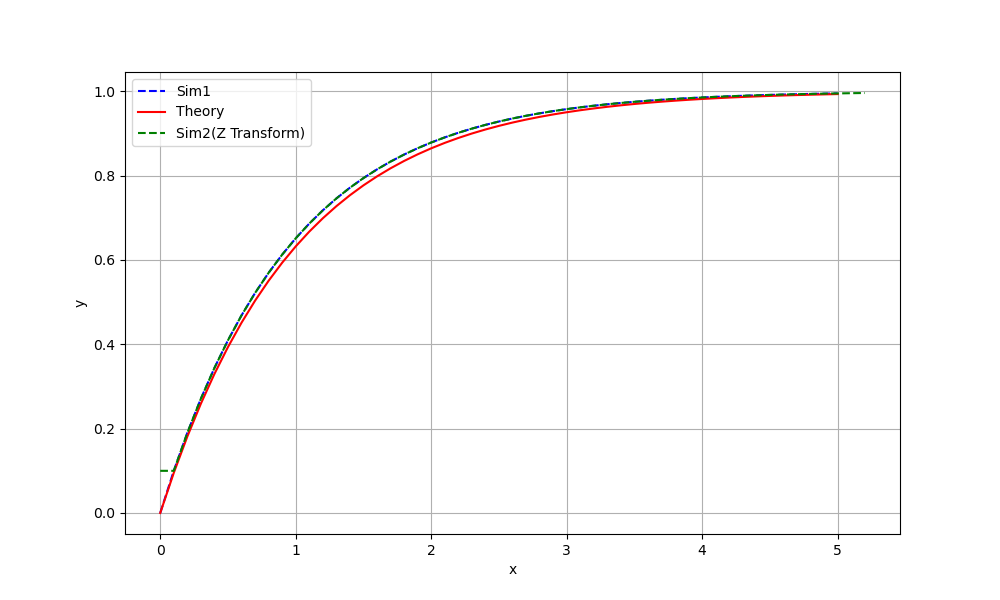
\includegraphics[width=0.7\columnwidth]{figs/Q1.png}
    \label{stemplot}
\end{figure}
\end{frame}


\end{document}

